\documentclass[a4paper,12pt]{scrreprt}

\usepackage[utf8x]{inputenc}
\usepackage{ucs}
\usepackage{graphicx}
\usepackage[ngerman]{babel}
\usepackage{acronym}
\usepackage{eurosym}
\usepackage[linktocpage=true]{hyperref}
\usepackage{caption}
\captionsetup{format=hang, justification=raggedright}
\usepackage[sort]{natbib} % vgl. http://merkel.zoneo.net/Latex/natbib.php

\setcounter{secnumdepth}{4}
\setcounter{tocdepth}{4}


\begin{document}

\pagenumbering{gobble} % seitenzahlnummerierung unterdrücken

% evtl. Sperrvermerkseite
Falls erforderlich (nur in begründeten Fällen): Sperrvermerk


% Titelblatt:
\newpage
\pagenumbering{arabic} % seitenzahlnummerierung ab hier beginnen
\begin{titlepage}
  \mbox{}
  \vspace{5mm}
  \begin{center}
    \huge{\textbf{\sffamily[TITEL DER ARBEIT]}} \\
    \huge{\textbf{\sffamily[evtl. Untertitel]}}\\
  \end{center}
  \vspace{40mm}
  \begin{flushright}
  Bachelorarbeit [1 bzw. 2 anführen]\\
  zur Erlangung des akademischen Grades\\
  Bachelor of Science in Engineering (BSc)

  \vspace{20mm}
  Fachhochschule Vorarlberg\\
  Mechatronics

  \vspace{40mm}
  Betreut von\\\relax
  [akad. Grad Name Betreuer/in anführen]\\
  Vorgelegt von\\\relax
  [(sofern vorhanden akad. Grad\footnote{Bitte beachten Sie, dass akademische Grade nach dem gestuften System nach dem Namen, getrennt durch ein Komma, gesetzt werden}) Name Studierende/r anführen]\\

  \vspace{20mm}
  Dornbirn, [Monat Jahr anführen]
  \end{flushright}
\end{titlepage}


% evtl. Widmung:
\chapter*{[Evtl. Widmung]}


% Abstract:
\newpage
\chapter*{Abstract}
[Englischen Titel anführen]

Formatvorlage für den Fließtext.


% Kurzreferat:
\newpage
\chapter*{Kurzreferat}
[Deutschen Titel anführen]

Formatvorlage für den Fließtext.

Lorem ipsum dolor sit amet, consetetur sadipscing elitr, sed diam nonumy
eirmod tempor invidunt ut labore et dolore magna aliquyam erat, sed diam
voluptua. At vero eos et accusam et justo duo dolores et ea rebum. Stet
clita kasd gubergren, no sea takimata sanctus est Lorem ipsum dolor sit
amet. Lorem ipsum dolor sit amet, consetetur sadipscing elitr, sed diam
nonumy eirmod tempor invidunt ut labore et dolore magna aliquyam erat, sed
diam voluptua. At vero eos et accusam et justo duo dolores et ea rebum.
Stet clita kasd gubergren, no sea takimata sanctus est Lorem ipsum dolor
sit amet.


% evtl. Vorwort:
\newpage
\chapter*{[Evtl. Vorwort]}

\tableofcontents

\clearpage
\phantomsection
\addcontentsline{toc}{chapter}{Abbildungsverzeichnis}
\listoffigures

\clearpage
\phantomsection
\addcontentsline{toc}{chapter}{Tabellenverzeichnis}
\listoftables


% evtl. Abkürzungsverzeichnis:
\newpage
\chapter*{[Bei Bedarf Abkürzungsverzeichnis]}
\begin{acronym}[SQL]
 \acro{KDE}{K Desktop Environment}
 \acro{SQL}{Structured Query Language}
 \acro{Bash}{Bourne-again shell}
\end{acronym}

% reference to the 'content' folder
% define and add/include you chapters and/or sections here.
% be aware though, paths are relative to 'main.tex'
\chapter{Einleitung}
Lorem ipsum dolor sit amet, consetetur sadipscing elitr, sed diam nonumy
eirmod tempor invidunt ut labore et dolore magna aliquyam erat, sed diam
voluptua. At vero eos et accusam et justo duo dolores et ea rebum. Stet
clita kasd gubergren, no sea takimata sanctus est Lorem ipsum dolor sit
amet. Lorem ipsum dolor sit amet, consetetur sadipscing elitr, sed diam
nonumy eirmod tempor invidunt ut labore et dolore magna aliquyam erat, sed
diam voluptua. At vero eos et accusam et justo duo dolores et ea rebum.
Stet clita kasd gubergren, no sea takimata sanctus est Lorem ipsum dolor
sit amet.

\begin{quote}

  Formatvorlage für ein längeres direktes Zitat. Formatvorlage für ein
  längeres direktes Zitat. Formatvorlage für ein längeres direktes Zitat.
  Formatvorlage für ein längeres direktes Zitat. Formatvorlage für ein
  längeres direktes Zitat. Formatvorlage für ein längeres direktes Zitat….

\end{quote}

Hinweise zum Zitieren und Belegen fremder Quellen finden Sie in der
Lehrunterlage \glqq Wissenschaftliches Arbeiten. Ein Leitfaden\grqq. Die
aktuelle Fassung dieses Leitfadens ist auf der FHV-Bibliothekshomepage
hinterlegt und kann frei heruntergeladen werden (\href{http://www.fhv.at/bibliothek/teaching-library/leitfaden}{http://www.fhv.at/bibliothek/teaching-library/leitfaden}).

\chapter{Hauptteil}
Lorem ipsum dolor sit amet, consetetur sadipscing elitr, sed diam nonumy
eirmod...

Hier eine Liste.
\begin{enumerate}
 \item Verstehen
 \item Üben
 \item Können
\end{enumerate}


\section{Unterkapitel zweite Ebene}
Formatvorlage für den Fließtext. Die Abbildung~\ref{fig:ex} auf Seite \pageref{fig:ex} zeigt drei Entladungskurven eines biphasischen Defibrillators.
\begin{figure}[htb]
  \centering
  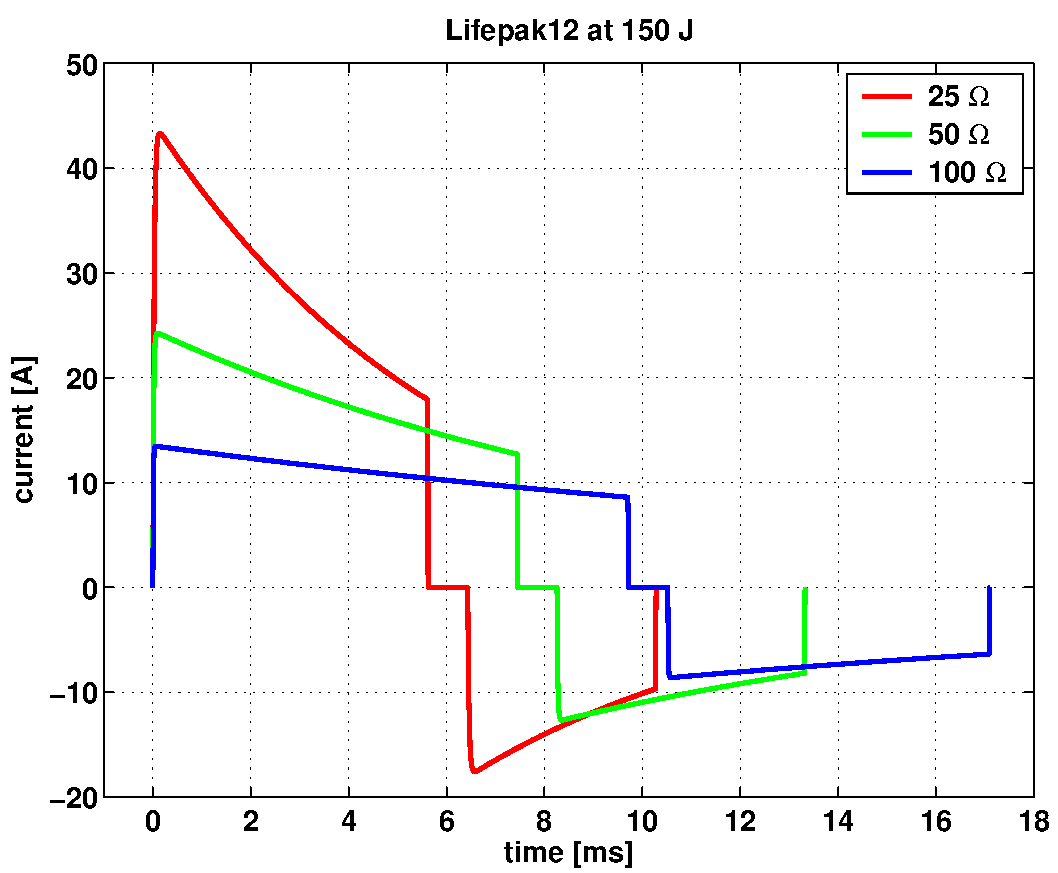
\includegraphics[width=6cm]{content/image/defi}
  \caption[Entladungskurven eines biphasischen Defibrillators]{Drei Entladungskurven. \\Quelle: eigene Ausarbeitung}
 \label{fig:ex}
\end{figure}


\section{Unterkapitel zweite Ebene}
Formatvorlage für den Fließtext.
Jetzt eine Fußnote\footnote{Dies ist eine Fußnote.}
Die quadratischen Gleichung (\ref{equ:foo}) hat wieviele Nullstellen?
\begin{equation}
 \label{equ:foo}
 x^2-2x+5=0.
\end{equation}
Zwei von Einsteins berühmtesten Formeln lauten:
\begin{eqnarray*}
  E &= mc^2                                  \\
  m &= \frac{m_0}{\sqrt{1-\frac{v^2}{c^2}}}
\end{eqnarray*}


\subsection{Unterkapitel dritte Ebene}
Formatvorlage für den Fließtext. Hier die einfache Tabelle \ref{tab:sp}

\begin{table}[htb]
  \centering
  \begin{tabular}{ | l | l |c|}
    \hline
    Datum      & Thema           & Raum \\
    \hline\hline
    Montag     & Graphentheorie  & U1   \\
    \hline
    Donnerstag & Algebra         & MZB23\\
    \hline
  \end{tabular}
  \caption[Stundenplan]{Stundenplan des Jahres 2030.\\ Quelle: eigene Ausarbeitung}
  \label{tab:sp}
\end{table}

\subsubsection{Unterkapitel vierte Ebene}
Formatvorlage für den Fließtext.

\paragraph{Unterkapitel fünfte Ebene}\mbox{}\newline
Formatvorlage für den Fließtext.

\paragraph{Unterkapitel fünfte Ebene}\mbox{}\newline
Formatvorlage für den Fließtext.


\section{Unterkapitel zweite Ebene}
Formatvorlage für den Fließtext.
Hier ein gutes Buch \citep[vgl.][Kapitel 2]{Chvatal1983} und dieser interessante Artikel \citep{Einstein1905} eines berühmten Herrn.


\chapter{[Weiteres Kapitel des Hauptteils]}

\section{Unterkapitel zweite Ebene}
Formatvorlage für den Fließtext.

\subsection{Unterkapitel dritte Ebene}
Formatvorlage für den Fließtext.

\subsubsection{Unterkapitel vierte Ebene}
Formatvorlage für den Fließtext.

\paragraph{Unterkapitel fünfte Ebene}\mbox{}\newline
Formatvorlage für den Fließtext.

\paragraph{Unterkapitel fünfte Ebene}\mbox{}\newline
Formatvorlage für den Fließtext.


\chapter{[Abschließende(s) Kapitel]}
Formatvorlage für den Fließtext.



% \bibliographystyle{unsrt}
% \bibliographystyle{alpha}
% \bibliographystyle{plain}
% \bibliographystyle{unsrtnat}
\bibliographystyle{authordate3}
\clearpage
\phantomsection
\addcontentsline{toc}{chapter}{Literaturverzeichnis}
\bibliography{references} % references.bib ist die verwendete bibtex-datei


\chapter*{[Evtl. Anhang]}
\addcontentsline{toc}{chapter}{[Evtl. Anhang]}
Formatvorlage für den Fließtext.


\chapter*{Eidesstattliche Erklärung}
\addcontentsline{toc}{chapter}{Eidesstattliche Erklärung}
Ich erkläre hiermit an Eides statt, dass ich die vorliegende Bachelorarbeit selbstständig und ohne Benutzung anderer als der angegebenen Hilfsmittel angefertigt habe. Die aus fremden Quellen direkt oder indirekt übernommenen Stellen sind als solche kenntlich gemacht. Die Arbeit wurde bisher weder in gleicher noch in ähnlicher Form einer anderen Prüfungsbehörde vorgelegt und auch noch nicht veröffentlicht.

\vspace{30mm}
\noindent
Verfasser/in\hfill                                       Unterschrift Verfasser/in

\vspace{3mm}
\noindent
Dornbirn, am [Tag. Monat Jahr anführen]\hfill            Vor- und Nachname Verfasser/in


\end{document}
